% Cover letter: Research Assistant (Remote), AI facial data collection (recruiter, client not named)
% CV: Sections/cv_research_assistant.tex -> cv_gen/cv_giovanni_tauro-research_assistant_facial_data.pdf
\documentclass[11pt,a4paper,sans]{moderncv}
% Shared preamble and header for the cover letters.
% One main file per application: cl_<company>.tex, built to
% cv_gen/coverletter_giovanni_tauro-<company>.pdf next to cv_giovanni_tauro-<company>.pdf.
% Paths (cl_gen/..., Pictures/...) are relative to the project root, as in the CV (see .latexmkrc).

\moderncvstyle{classic}
\moderncvcolor{blue}

\usepackage[scale=0.80]{geometry}
\setlength{\footskip}{136.00005pt}

\usepackage{fontawesome5}
% hyperref is loaded by moderncv itself; loading it here causes an option clash
\usepackage{xcolor}
\usepackage{graphicx}
\ifxetexorluatex
  \usepackage{fontspec}
  \usepackage{unicode-math}
  \defaultfontfeatures{Ligatures=TeX}
  \setmainfont{Latin Modern Roman}
  \setsansfont{Latin Modern Sans}
  \setmonofont{Latin Modern Mono}
  \setmathfont{Latin Modern Math}
\else
  \usepackage[T1]{fontenc}
  \usepackage{lmodern}
\fi

\usepackage[english]{babel}

% used for the PDF title and the letter closing; the visible header is \clheader below
\name{Giovanni}{Tauro}

% Header: #1 = headline under the name (same as the headline of the matching CV)
\newcommand{\clheader}[1]{%
\noindent
\begin{minipage}[c]{0.74\textwidth}
    {\Huge \textbf{Giovanni Tauro}}\\[-0.2em]
    {\small #1}\\[0.3em]

    \footnotesize
    \faMapMarker*~
    \href{https://www.google.com/maps/search/?api=1&query=Lecco+23900+Italy}
    {\color{blue}Bari-Lecco, Italy}
    \quad
    \faPhone*~
    \href{https://wa.me/393279437161}
    {\color{blue}+39 3279437161}
    \quad
    \faEnvelope~
    \href{mailto:giovanni.taurodi@gmail.com}
    {\color{blue}giovanni.taurodi@gmail.com}
    \\[-0.1em]

    \faLinkedin~
    \href{https://www.linkedin.com/in/giovanni-tauro-gt/}
    {\color{blue}LinkedIn}
    \quad
    \faGithub~
    \href{https://github.com/jotades}
    {\color{blue}GitHub}
    \quad
    \faGraduationCap~
    \href{https://scholar.google.com/citations?user=BS0aVGgAAAAJ&hl=it}
    {\color{blue}Scholar}
    \quad
    \faFilePdf~
    \href{https://www.notion.so/Giovanni-Tauro-2a7901d92f3a800b892af425c5875c6a}
    {\color{blue}Portfolio}
    \quad
    \faCubes~
    \href{https://grabcad.com/giovanni.tauro-3}
    {\color{blue}GrabCAD}

\end{minipage}
\hfill
\begin{minipage}[c]{0.18\textwidth}
    \raggedleft
    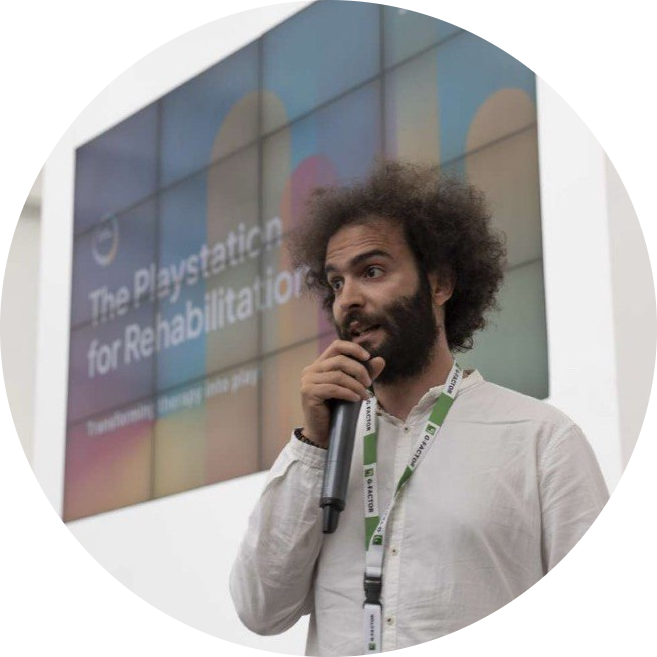
\includegraphics[width=2.8cm]{Pictures/Giovanni_pitch}
\end{minipage}
\vspace{0.1em}
}

\makeatletter
% the sender details are already in \clheader, so skip moderncv's own block
\@detailsfalse
% closing phrase, signature, name
\renewcommand*{\makeletterclosing}{%
  \@closing\\[0.6em]%
  
\includegraphics[height=1.2cm]{Pictures/sign_gt.jpg}\\[0.2em]%
  {\bfseries\@firstname~\@lastname}}
\makeatother


\begin{document}

\clheader{R\&D Engineer, PhD Candidate | Experimental Data \& Sensing}

\recipient{Recruitment Team}{Research Assistant (Remote)}
\opening{Dear Hiring Team,}
\closing{Yours faithfully,}
\makelettertitle

I am applying for the Research Assistant (Remote) position in AI facial data collection. I am an R\&D engineer and PhD candidate with more than five years of applied research at CNR-STIIMA, the Italian National Research Council, where collecting reliable data from people is a central part of my work.

For my PhD project, OmniTrack, I collected and validated position (x, y, z) and IMU data from 16 blind participants under experimental protocols. I was responsible for the whole chain: setting up the sensors, running the sessions, checking the quality of each recording, keeping the logs and analysing the data in Python. I have not collected facial images before, but the discipline is the same: a clear protocol, consistent capture conditions, accurate metadata and a record of every session that can be audited later.

I also understand what the data is for. I have built embedded machine-learning classifiers with TensorFlow Lite, so I know how the quality, variety and labelling of a dataset decide how well a model performs, and why a diverse sample matters.

My studies involve human participants, including blind adults and children in clinical settings, so I am used to working with informed consent and personal data under GDPR.

I work well on my own. I have carried out research stays at Utrecht University and Toyo University in Tokyo, and I am used to organising my work and reporting to teams in other countries with little supervision.

I would be glad to discuss the role further.

\makeletterclosing

\end{document}
